\icode{N16-MM-MU-L3-261014-001}
\nceeID[6]{2016新课标\Rmnum{3}}{19}
如图，一固定容器的内壁是半径为\(R\)的半球面；在半球面水平直径的一端有一质量为\(m\)的质点\(P\)。它在容器内壁由静止下滑到最低点的过程中，克服摩擦力做的功为\(W\)。重力加速度大小为\(g\)。设质点\(P\)在最低点时，向心加速度的大小为\(a\)，容器对它的支持力大小为\(N\)，则\paren[]

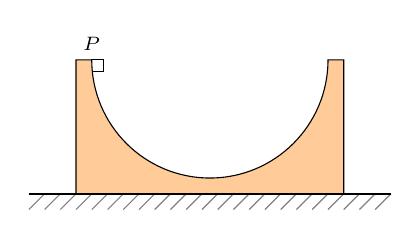
\begin{tikzpicture}[font=\scriptsize]
	\draw (0,0)node[above]{\(P\)} rectangle(.15,-.15);
	\draw[fill=orange!40] (-.2,-1.7)--(-.2,0)--(0,0) arc(-180:0:1.5)--(3.2,0)--(3.2,-1.7);
	\foreach \x in {-.8,-.6,...,3.6}
		\draw[gray] (\x,-1.9)--++(.2,.2);
	\draw[thick] (-.8,-1.7)--(3.8,-1.7);
\end{tikzpicture}
\begin{choices}
	\item\(a = \dfrac{2(mgR - W)}{mR}\)
	\item\(a = \dfrac{2mgR - W}{mR}\)
	\item\(N = \dfrac{3mgR - W}{R}\)
	\item\(N = \dfrac{2(mgR - W)}{R}\)
\end{choices}
\begin{answer}
    AC\qquad 提示：计算向心力时应用相对速度
\end{answer}